%% bare_jrnl.tex
%% V1.4b
%% 2015/08/26
%% by Michael Shell
%% see http://www.michaelshell.org/
%% for current contact information.
%%
%% This is a skeleton file demonstrating the use of IEEEtran.cls
%% (requires IEEEtran.cls version 1.8b or later) with an IEEE
%% journal paper.
%%
%% Support sites:
%% http://www.michaelshell.org/tex/ieeetran/
%% http://www.ctan.org/pkg/ieeetran
%% and
%% http://www.ieee.org/

%%*************************************************************************
%% Legal Notice:
%% This code is offered as-is without any warranty either expressed or
%% implied; without even the implied warranty of MERCHANTABILITY or
%% FITNESS FOR A PARTICULAR PURPOSE! 
%% User assumes all risk.
%% In no event shall the IEEE or any contributor to this code be liable for
%% any damages or losses, including, but not limited to, incidental,
%% consequential, or any other damages, resulting from the use or misuse
%% of any information contained here.
%%
%% All comments are the opinions of their respective authors and are not
%% necessarily endorsed by the IEEE.
%%
%% This work is distributed under the LaTeX Project Public License (LPPL)
%% ( http://www.latex-project.org/ ) version 1.3, and may be freely used,
%% distributed and modified. A copy of the LPPL, version 1.3, is included
%% in the base LaTeX documentation of all distributions of LaTeX released
%% 2003/12/01 or later.
%% Retain all contribution notices and credits.
%% ** Modified files should be clearly indicated as such, including  **
%% ** renaming them and changing author support contact information. **
%%*************************************************************************


% *** Authors should verify (and, if needed, correct) their LaTeX system  ***
% *** with the testflow diagnostic prior to trusting their LaTeX platform ***
% *** with production work. The IEEE's font choices and paper sizes can   ***
% *** trigger bugs that do not appear when using other class files.       ***                          ***
% The testflow support page is at:
% http://www.michaelshell.org/tex/testflow/



\documentclass[journal]{IEEEtran}
%
% If IEEEtran.cls has not been installed into the LaTeX system files,
% manually specify the path to it like:
% \documentclass[journal]{../sty/IEEEtran}





% Some very useful LaTeX packages include:
% (uncomment the ones you want to load)


% *** MISC UTILITY PACKAGES ***
%
%\usepackage{ifpdf}
% Heiko Oberdiek's ifpdf.sty is very useful if you need conditional
% compilation based on whether the output is pdf or dvi.
% usage:
% \ifpdf
%   % pdf code
% \else
%   % dvi code
% \fi
% The latest version of ifpdf.sty can be obtained from:
% http://www.ctan.org/pkg/ifpdf
% Also, note that IEEEtran.cls V1.7 and later provides a builtin
% \ifCLASSINFOpdf conditional that works the same way.
% When switching from latex to pdflatex and vice-versa, the compiler may
% have to be run twice to clear warning/error messages.






% *** CITATION PACKAGES ***
%
\usepackage{cite}
% cite.sty was written by Donald Arseneau
% V1.6 and later of IEEEtran pre-defines the format of the cite.sty package
% \cite{} output to follow that of the IEEE. Loading the cite package will
% result in citation numbers being automatically sorted and properly
% "compressed/ranged". e.g., [1], [9], [2], [7], [5], [6] without using
% cite.sty will become [1], [2], [5]--[7], [9] using cite.sty. cite.sty's
% \cite will automatically add leading space, if needed. Use cite.sty's
% noadjust option (cite.sty V3.8 and later) if you want to turn this off
% such as if a citation ever needs to be enclosed in parenthesis.
% cite.sty is already installed on most LaTeX systems. Be sure and use
% version 5.0 (2009-03-20) and later if using hyperref.sty.
% The latest version can be obtained at:
% http://www.ctan.org/pkg/cite
% The documentation is contained in the cite.sty file itself.






% *** GRAPHICS RELATED PACKAGES ***
%
\ifCLASSINFOpdf
  \usepackage[pdftex]{graphicx}
  % declare the path(s) where your graphic files are
  % \graphicspath{{../pdf/}{../jpeg/}}
  % and their extensions so you won't have to specify these with
  % every instance of \includegraphics
  % \DeclareGraphicsExtensions{.pdf,.jpeg,.png}
\else
  % or other class option (dvipsone, dvipdf, if not using dvips). graphicx
  % will default to the driver specified in the system graphics.cfg if no
  % driver is specified.
  \usepackage[dvips]{graphicx}
  % declare the path(s) where your graphic files are
  % \graphicspath{{../eps/}}
  % and their extensions so you won't have to specify these with
  % every instance of \includegraphics
  % \DeclareGraphicsExtensions{.eps}
\fi
% graphicx was written by David Carlisle and Sebastian Rahtz. It is
% required if you want graphics, photos, etc. graphicx.sty is already
% installed on most LaTeX systems. The latest version and documentation
% can be obtained at: 
% http://www.ctan.org/pkg/graphicx
% Another good source of documentation is "Using Imported Graphics in
% LaTeX2e" by Keith Reckdahl which can be found at:
% http://www.ctan.org/pkg/epslatex
%
% latex, and pdflatex in dvi mode, support graphics in encapsulated
% postscript (.eps) format. pdflatex in pdf mode supports graphics
% in .pdf, .jpeg, .png and .mps (metapost) formats. Users should ensure
% that all non-photo figures use a vector format (.eps, .pdf, .mps) and
% not a bitmapped formats (.jpeg, .png). The IEEE frowns on bitmapped formats
% which can result in "jaggedy"/blurry rendering of lines and letters as
% well as large increases in file sizes.
%
% You can find documentation about the pdfTeX application at:
% http://www.tug.org/applications/pdftex





% *** MATH PACKAGES ***
%
% \usepackage{amsmath}
% A popular package from the American Mathematical Society that provides
% many useful and powerful commands for dealing with mathematics.
%
% Note that the amsmath package sets \interdisplaylinepenalty to 10000
% thus preventing page breaks from occurring within multiline equations. Use:
% \interdisplaylinepenalty=2500
% after loading amsmath to restore such page breaks as IEEEtran.cls normally
% does. amsmath.sty is already installed on most LaTeX systems. The latest
% version and documentation can be obtained at:
% http://www.ctan.org/pkg/amsmath





% *** SPECIALIZED LIST PACKAGES ***
%
%\usepackage{algorithmic}
% algorithmic.sty was written by Peter Williams and Rogerio Brito.
% This package provides an algorithmic environment for describing algorithms.
% You can use the algorithmic environment in-text or within a figure
% environment to provide for a floating algorithm. Do NOT use the algorithm
% floating environment provided by algorithm.sty (by the same authors) or
% algorithm2e.sty (by Christophe Fiorio) as the IEEE does not use dedicated
% algorithm float types and packages that provide these will not provide
% correct IEEE style captions. The latest version and documentation of
% algorithmic.sty can be obtained at:
% http://www.ctan.org/pkg/algorithms
% Also of interest may be the (relatively newer and more customizable)
% algorithmicx.sty package by Szasz Janos:
% http://www.ctan.org/pkg/algorithmicx




% *** ALIGNMENT PACKAGES ***
%
\usepackage{array}
% Frank Mittelbach's and David Carlisle's array.sty patches and improves
% the standard LaTeX2e array and tabular environments to provide better
% appearance and additional user controls. As the default LaTeX2e table
% generation code is lacking to the point of almost being broken with
% respect to the quality of the end results, all users are strongly
% advised to use an enhanced (at the very least that provided by array.sty)
% set of table tools. array.sty is already installed on most systems. The
% latest version and documentation can be obtained at:
% http://www.ctan.org/pkg/array


% IEEEtran contains the IEEEeqnarray family of commands that can be used to
% generate multiline equations as well as matrices, tables, etc., of high
% quality.




% *** SUBFIGURE PACKAGES ***
%\ifCLASSOPTIONcompsoc
%  \usepackage[caption=false,font=normalsize,labelfont=sf,textfont=sf]{subfig}
%\else
%  \usepackage[caption=false,font=footnotesize]{subfig}
%\fi
% subfig.sty, written by Steven Douglas Cochran, is the modern replacement
% for subfigure.sty, the latter of which is no longer maintained and is
% incompatible with some LaTeX packages including fixltx2e. However,
% subfig.sty requires and automatically loads Axel Sommerfeldt's caption.sty
% which will override IEEEtran.cls' handling of captions and this will result
% in non-IEEE style figure/table captions. To prevent this problem, be sure
% and invoke subfig.sty's "caption=false" package option (available since
% subfig.sty version 1.3, 2005/06/28) as this is will preserve IEEEtran.cls
% handling of captions.
% Note that the Computer Society format requires a larger sans serif font
% than the serif footnote size font used in traditional IEEE formatting
% and thus the need to invoke different subfig.sty package options depending
% on whether compsoc mode has been enabled.
%
% The latest version and documentation of subfig.sty can be obtained at:
% http://www.ctan.org/pkg/subfig




% *** FLOAT PACKAGES ***
%
%\usepackage{fixltx2e}
% fixltx2e, the successor to the earlier fix2col.sty, was written by
% Frank Mittelbach and David Carlisle. This package corrects a few problems
% in the LaTeX2e kernel, the most notable of which is that in current
% LaTeX2e releases, the ordering of single and double column floats is not
% guaranteed to be preserved. Thus, an unpatched LaTeX2e can allow a
% single column figure to be placed prior to an earlier double column
% figure.
% Be aware that LaTeX2e kernels dated 2015 and later have fixltx2e.sty's
% corrections already built into the system in which case a warning will
% be issued if an attempt is made to load fixltx2e.sty as it is no longer
% needed.
% The latest version and documentation can be found at:
% http://www.ctan.org/pkg/fixltx2e


%\usepackage{stfloats}
% stfloats.sty was written by Sigitas Tolusis. This package gives LaTeX2e
% the ability to do double column floats at the bottom of the page as well
% as the top. (e.g., "\begin{figure*}[!b]" is not normally possible in
% LaTeX2e). It also provides a command:
%\fnbelowfloat
% to enable the placement of footnotes below bottom floats (the standard
% LaTeX2e kernel puts them above bottom floats). This is an invasive package
% which rewrites many portions of the LaTeX2e float routines. It may not work
% with other packages that modify the LaTeX2e float routines. The latest
% version and documentation can be obtained at:
% http://www.ctan.org/pkg/stfloats
% Do not use the stfloats baselinefloat ability as the IEEE does not allow
% \baselineskip to stretch. Authors submitting work to the IEEE should note
% that the IEEE rarely uses double column equations and that authors should try
% to avoid such use. Do not be tempted to use the cuted.sty or midfloat.sty
% packages (also by Sigitas Tolusis) as the IEEE does not format its papers in
% such ways.
% Do not attempt to use stfloats with fixltx2e as they are incompatible.
% Instead, use Morten Hogholm'a dblfloatfix which combines the features
% of both fixltx2e and stfloats:
%
% \usepackage{dblfloatfix}
% The latest version can be found at:
% http://www.ctan.org/pkg/dblfloatfix




%\ifCLASSOPTIONcaptionsoff
%  \usepackage[nomarkers]{endfloat}
% \let\MYoriglatexcaption\caption
% \renewcommand{\caption}[2][\relax]{\MYoriglatexcaption[#2]{#2}}
%\fi
% endfloat.sty was written by James Darrell McCauley, Jeff Goldberg and 
% Axel Sommerfeldt. This package may be useful when used in conjunction with 
% IEEEtran.cls'  captionsoff option. Some IEEE journals/societies require that
% submissions have lists of figures/tables at the end of the paper and that
% figures/tables without any captions are placed on a page by themselves at
% the end of the document. If needed, the draftcls IEEEtran class option or
% \CLASSINPUTbaselinestretch interface can be used to increase the line
% spacing as well. Be sure and use the nomarkers option of endfloat to
% prevent endfloat from "marking" where the figures would have been placed
% in the text. The two hack lines of code above are a slight modification of
% that suggested by in the endfloat docs (section 8.4.1) to ensure that
% the full captions always appear in the list of figures/tables - even if
% the user used the short optional argument of \caption[]{}.
% IEEE papers do not typically make use of \caption[]'s optional argument,
% so this should not be an issue. A similar trick can be used to disable
% captions of packages such as subfig.sty that lack options to turn off
% the subcaptions:
% For subfig.sty:
% \let\MYorigsubfloat\subfloat
% \renewcommand{\subfloat}[2][\relax]{\MYorigsubfloat[]{#2}}
% However, the above trick will not work if both optional arguments of
% the \subfloat command are used. Furthermore, there needs to be a
% description of each subfigure *somewhere* and endfloat does not add
% subfigure captions to its list of figures. Thus, the best approach is to
% avoid the use of subfigure captions (many IEEE journals avoid them anyway)
% and instead reference/explain all the subfigures within the main caption.
% The latest version of endfloat.sty and its documentation can obtained at:
% http://www.ctan.org/pkg/endfloat
%
% The IEEEtran \ifCLASSOPTIONcaptionsoff conditional can also be used
% later in the document, say, to conditionally put the References on a 
% page by themselves.




% *** PDF, URL AND HYPERLINK PACKAGES ***
%
\usepackage{url}
% url.sty was written by Donald Arseneau. It provides better support for
% handling and breaking URLs. url.sty is already installed on most LaTeX
% systems. The latest version and documentation can be obtained at:
% http://www.ctan.org/pkg/url
% Basically, \url{my_url_here}.



% *** GLOSSARIES AND ACRONYMNS ***
\usepackage[utf8]{inputenc}
\usepackage[acronym]{glossaries}
\makeglossaries

\newacronym{beta}{$\beta$}{Ratio of Venturi throat diameter, \acrshort{d}, to pipe diameter, \acrshort{D}}
\newacronym{expans}{$\varepsilon$}{Gas Expansibility Factor (see \cite{2003ISOTubes} section 5.6)}
\newacronym{RHOG}{$\rho_{1,gas}$}{Gas density at upstream tapping}
\newacronym{RHOL}{$\rho_{liquid}$}{Liquid density at upstream tapping}
\newacronym{WGC}{$\phi$}{Wet Gas Correction (WGC) parameter}
\newacronym{d}{$d$}{Venturi throat diameter}
\newacronym{D}{$D$}{Pipe diameter}
\newacronym{Frg}{$Fr_{gas}$}{Gas Froude Number, a dimensionless manner of representing gas velocity, $Fr_{gas}=\frac{v_{sg}}{\sqrt{gD}}\sqrt{\frac{\rho_{1,gas}}{\rho_{liquid}-\rho_{1,gas}}}$}
\newacronym{GMF}{GMF}{Gas Mass Fraction} 
\newacronym{GVF}{GVF}{Gas Volume Fraction}
\newacronym{H}{$H$}{H parameter from ISO/TR~11583:2012 \cite{2012ISO/TRConduits}}
\newacronym{PLR}{PLR}{Pressure Loss Ratio}
\newacronym{Q}{$Q$}{Flow rate, where $Q_{mg}$ is the gas mass flow rate, $Q_{ml}$ is the liquid mass flow rate, $Q_{vg}$ is the gas actual volume flow rate, $Q_{vl}$ is the liquid actual volume flow rate}
\newacronym{X}{$X$}{Lockhart-Martinelli parameter, $X=\frac{Q_{ml}}{Q_{mg}}\sqrt{\frac{\rho_{1,gas}}{\rho_{liquid}}}$}



\usepackage[font=footnotesize,justification=centering]{caption}
%\usepackage[font=footnotesize]{subcaption}
\usepackage{todonotes}

\usepackage{color,soul}  % Allows for text highlighting

% *** Do not adjust lengths that control margins, column widths, etc. ***
% *** Do not use packages that alter fonts (such as pslatex).         ***
% There should be no need to do such things with IEEEtran.cls V1.6 and later.
% (Unless specifically asked to do so by the journal or conference you plan
% to submit to, of course. )


% correct bad hyphenation here
\hyphenation{op-tical net-works semi-conduc-tor}


\begin{document}
%
% paper title
% Titles are generally capitalized except for words such as a, an, and, as,
% at, but, by, for, in, nor, of, on, or, the, to and up, which are usually
% not capitalized unless they are the first or last word of the title.
% Linebreaks \\ can be used within to get better formatting as desired.
% Do not put math or special symbols in the title.
\title{Evaluating characteristics of a Pressure Loss Ratio algorithm for horizontal wet gas Venturi meters
}
%
%
% author names and IEEE memberships
% note positions of commas and nonbreaking spaces ( ~ ) LaTeX will not break
% a structure at a ~ so this keeps an author's name from being broken across
% two lines.
% use \thanks{} to gain access to the first footnote area
% a separate \thanks must be used for each paragraph as LaTeX2e's \thanks
% was not built to handle multiple paragraphs
%

\author{Alistair~Collins\\
Development Engineer with Solartron ISA (Ametek)
% \thanks{}%
% \texttt{alistair.collins@ametek.com}
}


% The paper headers
\markboth{M101CEM CW1 Assignment, October-December 2018}%
{Shell \MakeLowercase{\textit{et al.}}: Bare Demo of IEEEtran.cls for IEEE Journals}
% The only time the second header will appear is for the odd numbered pages
% after the title page when using the twoside option.
% 
% *** Note that you probably will NOT want to include the author's ***
% *** name in the headers of peer review papers.                   ***
% You can use \ifCLASSOPTIONpeerreview for conditional compilation here if
% you desire.




% If you want to put a publisher's ID mark on the page you can do it like
% this:
%\IEEEpubid{0000--0000/00\$00.00~\copyright~2015 IEEE}
% Remember, if you use this you must call \IEEEpubidadjcol in the second
% column for its text to clear the IEEEpubid mark.



% use for special paper notices
%\IEEEspecialpapernotice{(Invited Paper)}




% make the title area
\maketitle

% As a general rule, do not put math, special symbols or citations
% in the abstract or keywords.
\begin{abstract}
The Pressure Loss Ratio from a Venturi meter provides an industrially robust method for quantifying the liquid content of high GVF multiphase flows. Key characteristics of the PLR algorithm from ISO/TR~11583:2012 are compared to experimental wet gas test data. Although general similarities in the PLR shape for increasing liquid content were noted, critical differences are also examined, with the improvements needed in particular for multi-liquid wet gas systems.
\end{abstract}


\section{Introduction}
\IEEEPARstart{V}{enturi} flow meters are an industrially proven technology for the metering of multiphase wet gas flow. Although Venturi wet gas correction methods originally borrowed from orifice plate corrections (for example, those by Murdock \cite{Murdock1962} and Chisholm \cite{Chisholm1977}), de Leeuw \cite{DeLeeuw1997} provided an ``empirical correlation...which accurately predicts the effect of the liquid phase on Venturi meter readings in wet gas horizontal flow.''  However, to utilize this correction to the gas rate, prior knowledge of the liquid rate is required, typically expressed through the Lockhart-Martinelli parameter, \acrshort{X}.\\

Within de Leeuw's paper \cite{DeLeeuw1997}, he indicates that there is ``potential for the pressure loss measurement...to use it as a means to determine the liquid content of the flow, from which the overreacting factor can be determined accordingly. In essence this would form a simple two-phase [i.e. wet gas] flow meter.''  The \acrlong{PLR} (PLR) is the overall difference in the pressure across the Venturi meter, $DP_{t}$ to that of the normal Venturi differential pressure, $DP_{v}$ :
\begin{equation}
    PLR = \frac{DP_{t}}{DP_{v}}
\end{equation}

This paper only uses data for the standard design for horizontal machined Venturi meters as given in ISO 5167-4:2003 \cite{2003ISOTubes}, whilst being suitable for wet gas (therefore not using annular chambers, pieziometer rings or triple-t tapping arrangements, or an upstream flow conditioner, as noted in section 11.1 of \cite{Reader-Harris2015}).  As such, the included angle of the inlet cone is $21^{\circ} \pm 1^{\circ}$; however, the standard included angle of the outlet cone may be set between $7^{\circ}$ and $15^{\circ}$.  Whereas the data from which the equations for ISO/TR 11583:2012 are drawn only allows for nominally $7^{\circ}$ outlet cones, the Dualstream 1 meters from Solartron ISA only have nominally $15^{\circ}$ outlet cones; overall this latter are shorter, but will have a different pressure recovery envelope.

\section{Related Work}
As has been mentioned above, de Leeuw \cite{DeLeeuw1997} recognized the potential for the \acrshort{PLR} to determine the liquid content of the wet gas flow, but was unable to provide an equation to formalize this relationship.

Direct modelling of the flow through a Venturi has been attempted, such as that by van Maanen and de Leeuw \cite{VanMaanen2016}, or by Yu et al. \cite{Yu2015}.  Whilst they provide useful information on the factors that influence wet gas flow through a Venturi, they lack (or do not disclose) a correlation or model for the meter that could be readily implemented to measure the multiphase wet gas flow.

However, Reader-Harris and Graham \cite{Reader-Harris2009} derived a new correlation for the wet gas correction term, \acrshort{WGC}, through using an extensive data set, extending the form used by Chisholm \cite{Chisholm1977} and de Leeuw \cite{DeLeeuw1997} through more complicated formulations for the discharge coefficient and the $n$ parameter.  An algorithmic relationship for the \acrshort{PLR} was also provided from a subset of this data (mostly 4" Venturi).  Both of these sets of equations are summarized in Appendix \ref{11583 Equations} below. Reader-Harris and Graham's work resulted in an ISO technical report, ISO/TR~11583:2012~\cite{2003ISOTubes}, which is also expanded upon in \cite{Reader-Harris2015}.  It is predominantly the calculation methods documented in the ISO report that are evaluated in this paper.

ISO/TR~11583:2012 received criticism from industry, including from de Leeuw, Steven and van Maanen \cite{DeLeeuw2011}, who noted that the \acrlong{PLR} for dry gas conditions does not well fit data at a wider range of Venturi size and \acrshort{beta} values than that used to develop the equations (but within the limits given in the standard).  Similarly, the effects of the water-to-liquid ratio on  \acrshort{PLR} are not taken into account, due in part to the lack of 3-phase data (simultaneous flow of gas, condensate and water) within the ISO/TR~11583:2012 data set: ``All aspects above lead to the conclusion that the statements made on the pressure loss ratio in the ISO report are incomplete and in some aspects incorrect.'' 

However, the potential for the \acrlong{PLR} remains, with Steven \cite{Steven2018OrificeProblem} subsequently noting that the \acrshort{PLR} could be a ``solution to the `Ill-posed' problem'', as a ``...wet gas flow’s liquid loading can be predicted via its relationship with the Venturi meter’s measureable Pressure Loss Ratio''.  Similarly, Pinguet \cite{Pinguet2018ExtensiveConditions} notes the use of the recovery pressure measurement as technique for determining the liquid loading, referencing the commercial implementation of Solartron ISA's Dualstream meters.

\section{Problem}

Whilst there is limited literature critically reviewing the form and accuracy of the equations presented in ISO/TR~11583:2012 for the use of \acrlong{PLR} with Venturi meters, a number of the comments by de Leeuw, Steven and van Maanen in section 8 of \cite{DeLeeuw2011} are particularly pertinent.  Those that are considered in this paper are listed below, specifically to determine whether the equations in the ISO Technical Report have the right form and the key characteristics.

\subsection{Evaluating the dry gas performance of \acrshort{PLR} for different flow meter sizes and beta ratios.}
From equation \ref{eq:11583_Y}, the measured \acrshort{PLR}, $\frac{\Delta \omega}{\Delta p}$, at dry gas conditions (when $Y=0$) is only proportional to beta; there are no terms for the meter size, gas-to-liquid density ratio, or gas velocity (which the gas densiometric Froude number, \acrshort{Frg}, represents in a non-dimensional manner).

\subsection{Evaluating the shape of the PLR equations}
Equations \ref{eq:11583_Ymax} and \ref{eq:11583_Y/Ymax} define the curves for \acrshort{PLR} as a plateauing exponential form for increasing liquid content, as given by the Lockhart-Martinelli number, $X$, (for constant density ratio, velocity and water-to-liquid ratio).

\subsection{Evaluating multiphase wet gas performance}
Multiphase wet gas (the flow of gas, condensate and water together) is only represented through the $H$ parameter.  de Leeuw, Steven and van Maanen did not consider this adaquate, noting, ``...the ISO report correlations neither align with other available experimental results nor describe realistic situations in which the liquid phase consists of condensate and water.''

\subsection{Sensitivity to pipe diameter at downstream tapping}
de Leeuw, Steven and van Maanen noted that ``...a demonstrated sensitivity of the pressure loss to the actual internal diameter of the pipe section where the pressure loss tapping is located...where the actual internal diameters of flow lines vary, this easily leads to significant changes in the total pressure loss ratio.''  It is therefore pertinent to confirm the diameter at the downstream tapping of the meters in the Solartron ISA database. 

\section{Solution}

Solartron ISA have an extensive wet gas calibration database for Venturi meters, which has previously been used to assess the performance of publicly available standard wet gas correlation algorithms \cite{Collins2015}.  Of relevance to this paper are 28 wet gas calibration projects (consisting of 5,418 test points in total, for meters nominally sized between 3" and 10") for Dualstream~1 products.

The total differential pressure may be measured to any point downstream of the Venturi, but the downstream tapping location (see figure \ref{fig:Venturi}) is generally either six pipe diameters - $6$\acrshort{D} - downstream of the end of the divergent cone (typical for standard meters, with the differential pressure given as $DP_{t6}$), or immediately after the divergent cone (i.e. a distance of zero pipe diameters - $0D$ - with a differential pressure of $DP_{t0}$, which is the downstream tapping location for Solartron~ISA's Dualstream~1 meters).

\begin{figure}[ht]
\centering
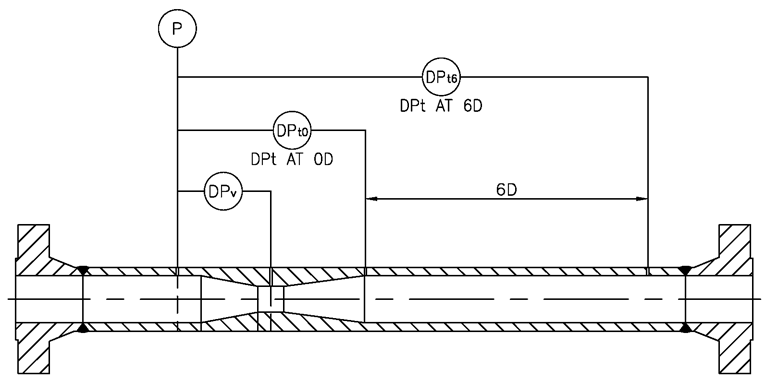
\includegraphics[width=3.4in]{Venturi.png}
\caption[]{ Venturi meter indicating pressure and differential pressure\\instrumentation }
\label{fig:Venturi}
\end{figure}

The positioning of the downstream tapping at $6D$ would appear to be due to the assumption that the pressure loss from the DP device would be fully recovered by this point, i.e. that further changes in the pressure would be dominated by the pipe frictional effects rather than the DP meter.  This may have been the expectation for an orifice plate meter, which has the vena contracta downstream of the plate, and therefore the pressure recovery does not start until then.  However, for the Venturi, the walls constrain the general shape of the flow, and a tapping at $6D$ may therefore be seen as a technological hangover from an alternative differential pressure meter.  For instance, Solartron ISA use $0D$ \cite{Collins2017PLR1}, believing it to provide similar information on the liquid phase in the flow meter, whilst also providing a higher (and therefore more readily measureable) $DP_{t}$.

The Solartron ISA database is therefore used to provide a ready comparison of the general features of the ISO Technical Report formulation by providing a source of instrumentation and reference data, without assuming the ISO equations will provide numerically accurate result.  Key characteristics of the PLR are therefore investigated to demonstrate the successes and limitations.

It is noted that in previous work \cite{Collins2015} the following formulation for the \acrshort{H} parameter in the ISO/TR~11583:2012 \cite{2012ISO/TRConduits} equations was used:

\begin{equation}
H = 1.0 + 0.35 \frac{Q_{mw}}{Q_{ml}}    
\end{equation}

This formula correctly implies that none of the data in the Solartron ISA database is for steam flow, and assumes a nominal straight line fit between the liquid being all hydrocarbon (where the water mass flow rate $Q_{mw}$ is zero) and all water, as was suggested by Graham in the paper presentation at the North Sea Flow Measurement conference.  However, Reader-Harris has more recently presented an alternative formulation \cite{Reader-Harris2017} based on evaluating futher three-phase data:

\begin{equation}
H = min \left( 1.0 + 0.8 \frac{Q_{vw}}{Q_{vl}}, 1.35 \right)    
\end{equation}

This uses the water-to-liquid volume ratio (WLR), and implies that the liquid fully behaves like water where $WLR~\geq~0.4375$, where this is attributed to the liquid mixture in this case having the surface tension of water.  Although this is a change from previous work, and is not within the ISO/TR~11583:2012 document, as the most recent suggestion of the paper authors, we have used this form within this paper.

\section{Analysis}

Whilst noting the key differences between the Venturi meters used for ISO/TR~11583:2012 and those of the Solartron ISA database (notably, the divergent cone angle and the distance of the downstream tapping from the exit of the divergent cone), figure \ref{fig:PLR2} provides an initial visual assessment of the performance of the ISO algorithms for this dataset (the red line indicating where the measured PLR equals that calculated by the ISO algorithms). This initial evaluation demonstrates that there appears to be a greater dependence upon the meter size - a parameter that is not explicitly used in the ISO formulation for \acrshort{PLR}. As the ISO equations for PLR are based only on 4" meters (with beta ratios of 0.4, 0.6 and 0.75 - see 11.3.2 in \cite{Reader-Harris2015}), this formulation is therefore unable to allow for this significant factor. 

\begin{figure}[h]
\centering
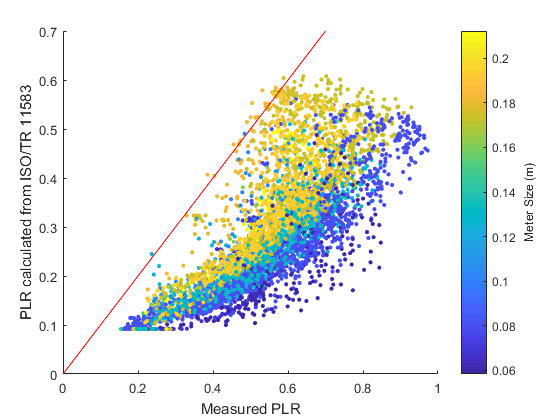
\includegraphics[width=3.4in]{PLR2.png}
\caption[]{ Measured PLR versus ISO/TR~11583:2012, coloured by meter size }
\label{fig:PLR2}
\end{figure}

As can also be seen in \ref{fig:PLRnaive}, a naive refitting of the ISO/TR~11583:2012 parameters to the Solartron ISA wet gas database, though resulting in a tighter correlation to the red line, still exhibits a dependence upon the meter size.  This is most clearly seen by comparing the dark blue points of the smallest meter (which tend towards the lower right of the chart), with those of the largest meter (which tend to upper left) - a clear trend in meter size, despite fitting to this specific dataset.

\begin{figure}[h]
\centering
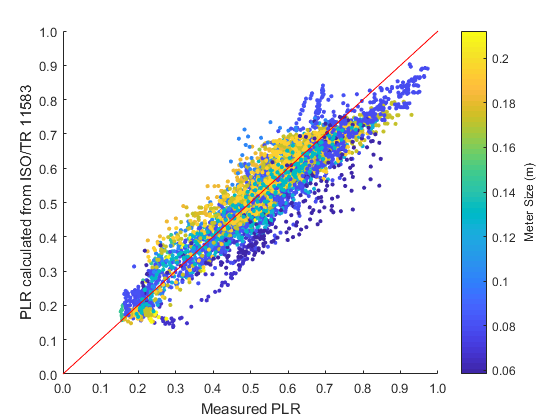
\includegraphics[width=3.4in]{PLRnaive.png}
\caption[]{ Measured PLR versus a naive refitting of ISO/TR~11583:2012, coloured by meter size }
\label{fig:PLRnaive}
\end{figure}

The natural conclusion of these analyses is that the formulation in the ISO Technical Report is unable to adequately represent the effect of meter size.  However, the proviso to that is the limitations of the Solartron ISA database, as it is possible - although considered unlikely - that with a downstream tapping at $6D$ and a lesser divergent cone angle this formulation would just work.

\subsection{Dry gas calibration data} 
The \acrshort{PLR} for dry gas data, according to ISO/TR~11583:2012, should only be proportional to beta, as per equation \ref{eq:11583_Y}.  The Solartron ISA database was used to investigate this assumption, with 383 dry gas points taken as part of wet gas tests available for analysis.  

Figures \ref{fig:4inchDry} and \ref{fig:6inchDry}, where each chart are at a fixed size and beta ratio, show that the dry gas PLR varies significantly, in contradiction to the ISO report.  The PLR value is seen to depend on the type of gas (nitrogen, air and natural gas data are shown), the gas density, and the gas Froude number.  However, clear trends (beyond higher gas Froude numbers tend to have higher PLR) are difficult to determine.

\begin{figure}[h]
\centering
\includegraphics[width=3.4in]{{"4inch dry"}.png}
\caption[]{ Dry gas data for 4" $0.55\beta$ Venturi (Nitrogen:~filled~circle, Natural~Gas:~empty~square) }
\label{fig:4inchDry}
\end{figure}

\begin{figure}[h]
\centering
\includegraphics[width=3.4in]{{"6inch dry"}.png}
\caption[]{ Dry gas data for 6" $0.55\beta$ Venturi (Nitrogen:~filled~circle, Air:~+, Natural~Gas:~empty~square) }
\label{fig:6inchDry}
\end{figure}

\subsection{Shape of PLR data}
Expanding upon the initial analysis above to compare the wet gas calibration data from the Solartron ISA database with the ISO/TR~11583:2012 equations for individual wet gas tests, it was assumed that the generic algorithmic shape given by the standard is comparable to that from the data.

For instance, figure \ref{fig:4inch0.55Wet} and \ref{fig:10inch0.55Wet} compares a representative sample of nominal 4" $0.55\beta$ and nominal 10" $0.55\beta$ \acrshort{PLR} data with the ISO/TR~11583:2012 calculations (for approximately constant gas density and gas flow rates).  Although there may initially appear to be significant differences, by linearly scaling the ISO results (as shown by the magenta values and line) it is apparent that the data is more readily comparable.  For greater alignment, a more complex scaling function would therefore be required.  As it stands, however, this data would appear to support Solartron ISA's belief that a PLR using a downstream tapping at $0D$ conveys much the same information as that of one at the "standard" $6D$ downstream of the Venturi's divergent cone.

\begin{figure}[h]
\centering
\includegraphics[width=3.4in]{{"4inch 0.55 PLR"}.png}
\caption[]{ Wet gas data for 4" $0.55\beta$ Venturi, comparing PLR data at 0D with ISO/TR~11583:2012 values at $6D$ and linearly scaled }
\label{fig:4inch0.55Wet}
\end{figure}

\begin{figure}[h]
\centering
\includegraphics[width=3.4in]{{"10inch 0.55 PLR"}.png}
\caption[]{ Wet gas data for 10" $0.55\beta$ Venturi, comparing PLR data at 0D with ISO/TR~11583:2012 values at $6D$ and linearly scaled }
\label{fig:10inch0.55Wet}
\end{figure}

\subsection{Multiphase wet gas data}
In the same manner, by evaluating data from a nominal 6" $0.55\beta$ at one gas density and gas flow rate for a number of water liquid ratios, as shown in figures \ref{fig:4inch0.55Wet2} and \ref{fig:6inch0.55Wet}, a similar comparison between the PLR data and the ISO results are shown. Comparable scaling is possible to provide greater alignment, although this is not shown in this figure.  However, it is apparent from figure \ref{fig:6inch0.55Wet} that the ISO/TR~11583:2012 formulation is not as good at the relative positioning of the intermediate water-liquid ratio data, as per the criticisms of \cite{DeLeeuw2011}.

\begin{figure}[h]
\centering
\includegraphics[width=3.4in]{{"4inch 0.55 PLR2"}.png}
\caption[]{ Wet gas data for 4" $0.55\beta$ Venturi, comparing PLR data at $0D$ with ISO/TR~11583:2012 values at $6D$ at different WLR }
\label{fig:4inch0.55Wet2}
\end{figure}

\begin{figure}[h]
\centering
\includegraphics[width=3.4in]{{"6inch 0.55 PLR"}.png}
\caption[]{ Wet gas data for 6" $0.55\beta$ Venturi, comparing PLR data at $0D$ with ISO/TR~11583:2012 values at $6D$ at different WLR }
\label{fig:6inch0.55Wet}
\end{figure}

\subsection{Pipe diameter at downstream tapping}
As the downstream tapping location of the Dualstream 1 meter is directly at the end of the divergent cone, the diameter is tightly controlled to be equal to the pipe diameter at the upstream tapping, confirmed via metrological testing.  This is a significant additional benefit to these meters in distinction to Venturi with the downstream tapping at $6D$, where there may be a fiscal reason for welding pipe of only nominally the same - or potentially even a different - diameter.


\section{Conclusions}

Whilst acknowledging the work of ISO/TR~11583:2012 \cite{2012ISO/TRConduits} as an initial step towards a comprehensive formulation for determining multiphase wet gas flow rates by using the Venturi \acrfull{PLR}, this paper indicates that further work is required to provide a truly generalized implementation.

Although the Solartron ISA wet gas calibration database uses Venturi meters with a greater outlet cone angle and an alternative total DP tapping location, this data has indicated a number of potential concerns.

With no clear dependence upon the meter size, the PLR equations from ISO/TR~11583:2012 appear insufficient to adequately represent the process data.  Even at dry gas conditions, the complexities of the meter size, gas Froude number and gas density do not appear to be adequately represented.

Similarly, test data indicates that the dependence of \acrshort{PLR} on the water-liquid ratio does not appear to be sufficient, as per previous criticism.

% Glossary
%\setglossarysection{section}
%\glsnogroupskiptrue
%\printglossary
%\printglossary[type=\acronymtype,nonumberlist,title=Glossary of Terms]

\section*{Glossary of Terms}

\begin{tabular}{p{0.6cm} p{7.3cm}}
$d$ & Venturi throat diameter. \\
$D$ & Pipe diameter. \\
$Fr_{g}$ &  Gas Froude number, a dimensionless representation of gas velocity. \\
& $Fr_{g} = \frac{v_{sg}}{\sqrt{gD}}\sqrt{\frac{\rho_{g}}{\rho_{l}-\rho_{g}}}$ \\
$H$ & $H$ parameter from ISO/TR~11583:2012 \cite{2012ISO/TRConduits}. \\
$PLR$ & Pressure Loss Ratio. \\
$X$ & Lockhart-Martinelli parameter, $X=\frac{Q_{ml}}{Q_{mg}}\sqrt{\frac{\rho_{1,gas}}{\rho_{liquid}}}$ \\
$\beta$ & Ratio of Venturi throat diameter, $d$, to pipe diameter, $D$. \\
$\phi$ & Wet Gas Correction (WGC) parameter.
\end{tabular}

\vfill\eject
% if have a single appendix:
%\appendix[Equations from ISO/TR 11583:2012]
% or
%\appendix  % for no appendix heading
% do not use \section anymore after \appendix, only \section*
% is possibly needed

% use appendices with more than one appendix
% then use \section to start each appendix
% you must declare a \section before using any
% \subsection or using \label (\appendices by itself
% starts a section numbered zero.)
%
\appendices
\section{Equations from ISO/TR 11583:2012} \label{11583 Equations}
%Appendix one text goes here.

ISO/TR 11583:2012\cite{2012ISO/TRConduits} (developed from \cite{Reader-Harris2009} and expanded upon in \cite{Reader-Harris2015}) provides a wet gas correction and \acrshort{PLR}-based determination of the liquid content.  A summary of the formulation is given below to allow for ready comparison in this paper.

\subsection{Determining the wet gas corrected gas mass flow rate $q_{m,gas}$}

\begin{equation}
    q_{m,gas} = \frac{C}{\sqrt{1-\beta^{4}}}\varepsilon\frac{\pi d^{2}}{4}\frac{\sqrt{2\Delta p \rho_{1,gas}}}{\phi}
\end{equation}

\begin{equation}
    C = 1 - 0.0463 e^{-0.05 Fr_{gas,th}} min \left( 1, \sqrt{\frac{X}{0.016}} \right )
\end{equation}

\begin{equation}
    X = \left( \frac{q_{m,liquid}}{q_{m,gas}} \right)\sqrt{\frac{\rho_{1,gas}}{\rho_{liquid}}}
\end{equation}

\begin{equation}
    Fr_{gas} = \frac{4q_{m,gas}}{\rho_{1,gas} \pi D^{2} \sqrt{gD}} \sqrt{\frac{\rho_{1,gas}}{\rho_{liquid}-\rho_{1,gas}}}
\end{equation}

\begin{equation}
    Fr_{gas,th} = \frac{Fr_{gas}}{\beta ^{2.5}}
\end{equation}

\begin{equation}
    \phi = \sqrt{1+C_{Ch}X+X^2}
\end{equation}

\begin{equation}
    C_{Ch} = \left( \frac{\rho_{liquid}}{\rho_{1,gas}} \right) ^{n} +\left( \frac{\rho_{1,gas}}{\rho_{liquid}} \right) ^{n}
\end{equation}

\begin{equation}
    n = max \left( 0.583 - 0.18 \beta^{2} - 0.578 e^{-0.8 \frac{Fr_{gas}}{H}}, 0.392 - 0.18 \beta^{2} \right)
\end{equation}
\\
$H = 1.0$ for hydrocarbon liquid,\\
$H = 1.35$ for water,\\
$H = 0.79$ for liquid water in wet-steam flow.
\\
\\
Limits of use: \\
\begin{equation*}
\begin{aligned}
    0.4 \leq \beta \leq 0.75 \\
    0 < X \leq 0.3 \\
    Fr_{gas,th} > 3 \\
    \frac{\rho_{1,gas}}{\rho_{liquid}} > 0.02 \\
    D \geq 50 mm
\end{aligned}
\end{equation*}



\subsection{For determining $X$ from the \acrshort{PLR}}

\begin{equation}
\label{eq:11583_Y}
    Y = \frac{\Delta \omega}{\Delta p} - 0.0896 -0.48 \beta^{9}
\end{equation}

\begin{equation}
\label{eq:11583_Ymax}
    Y_{max} = 0.61 exp \left( -11 \left( \frac{\rho_{1,gas}}{\rho_{liquid}} \right) - 0.045 \frac{Fr_{gas}}{H} \right)
\end{equation}

\begin{equation}
\label{eq:11583_Y/Ymax}
    \frac{Y}{Y_{max}} = 1 - exp \left(-35 X^{0.75} e^{-0.28 \frac{Fr_{gas}}{H}} \right)
\end{equation}
\\
Additional limits of use: \\
\begin{equation*}
\begin{aligned}
    Fr_{gas,th} > 4 \\
    \frac{Fr_{gas}}{H} \leq 5.5 \\
    \frac{\rho_{1,gas}}{\rho_{liquid}} \leq 0.09
\end{aligned}
\end{equation*}



% Can use something like this to put references on a page
% by themselves when using endfloat and the captionsoff option.
%\ifCLASSOPTIONcaptionsoff
%  \newpage
%\fi


\vfill\eject
% trigger a \newpage just before the given reference
% number - used to balance the columns on the last page
% adjust value as needed - may need to be readjusted if
% the document is modified later
% \IEEEtriggeratref{8}
% The "triggered" command can be changed if desired:
%\IEEEtriggercmd{\enlargethispage{-5in}}

% references section

% can use a bibliography generated by BibTeX as a .bbl file
% BibTeX documentation can be easily obtained at:
% http://mirror.ctan.org/biblio/bibtex/contrib/doc/
% The IEEEtran BibTeX style support page is at:
% http://www.michaelshell.org/tex/ieeetran/bibtex/
\bibliographystyle{IEEEtran}
% argument is your BibTeX string definitions and bibliography database(s)
\bibliography{references.bib}
%
% <OR> manually copy in the resultant .bbl file
% set second argument of \begin to the number of references
% (used to reserve space for the reference number labels box)
%\begin{thebibliography}{1}
%
%\bibitem{IEEEhowto:kopka}
%H.~Kopka and P.~W. Daly, \emph{A Guide to \LaTeX}, 3rd~ed.\hskip 1em plus
%  0.5em minus 0.4em\relax Harlow, England: Addison-Wesley, 1999.
%
%\end{thebibliography}

% use section* for acknowledgment
\section*{Acknowledgments}
The author would like to thank his supervision team at Coventry University (Erdal Turkbeyler, Seyed Shariatipour, Alban Potherat and Hoi Yeung), and Steve Clark and Mark Tudge of Solartron ISA (Ametek). 

% biography section
% 
% If you have an EPS/PDF photo (graphicx package needed) extra braces are
% needed around the contents of the optional argument to biography to prevent
% the LaTeX parser from getting confused when it sees the complicated
% \includegraphics command within an optional argument. (You could create
% your own custom macro containing the \includegraphics command to make things
% simpler here.)
%\begin{IEEEbiography}[{\includegraphics[width=1in,height=1.25in,clip,keepaspectratio]{mshell}}]{Michael Shell}
% or if you just want to reserve a space for a photo:

\begin{IEEEbiographynophoto}{Alistair Collins}
is a Development Engineer for Solartron~ISA (Ametek Oil \& Gas) since 2005, who manufacture the Dualstream range of wet gas flow meters.  He is currently undertaking an Engineering Doctorate in Flow Measurement and Fluid Mechanics at Coventry University.
\end{IEEEbiographynophoto}

\end{document}


